\setcounter{equation}{0}
\chapter{Sobre o candidato}
	\begin{figure}[h!]													% Begin of the figure
  		\centering														% Centering the figure
   			 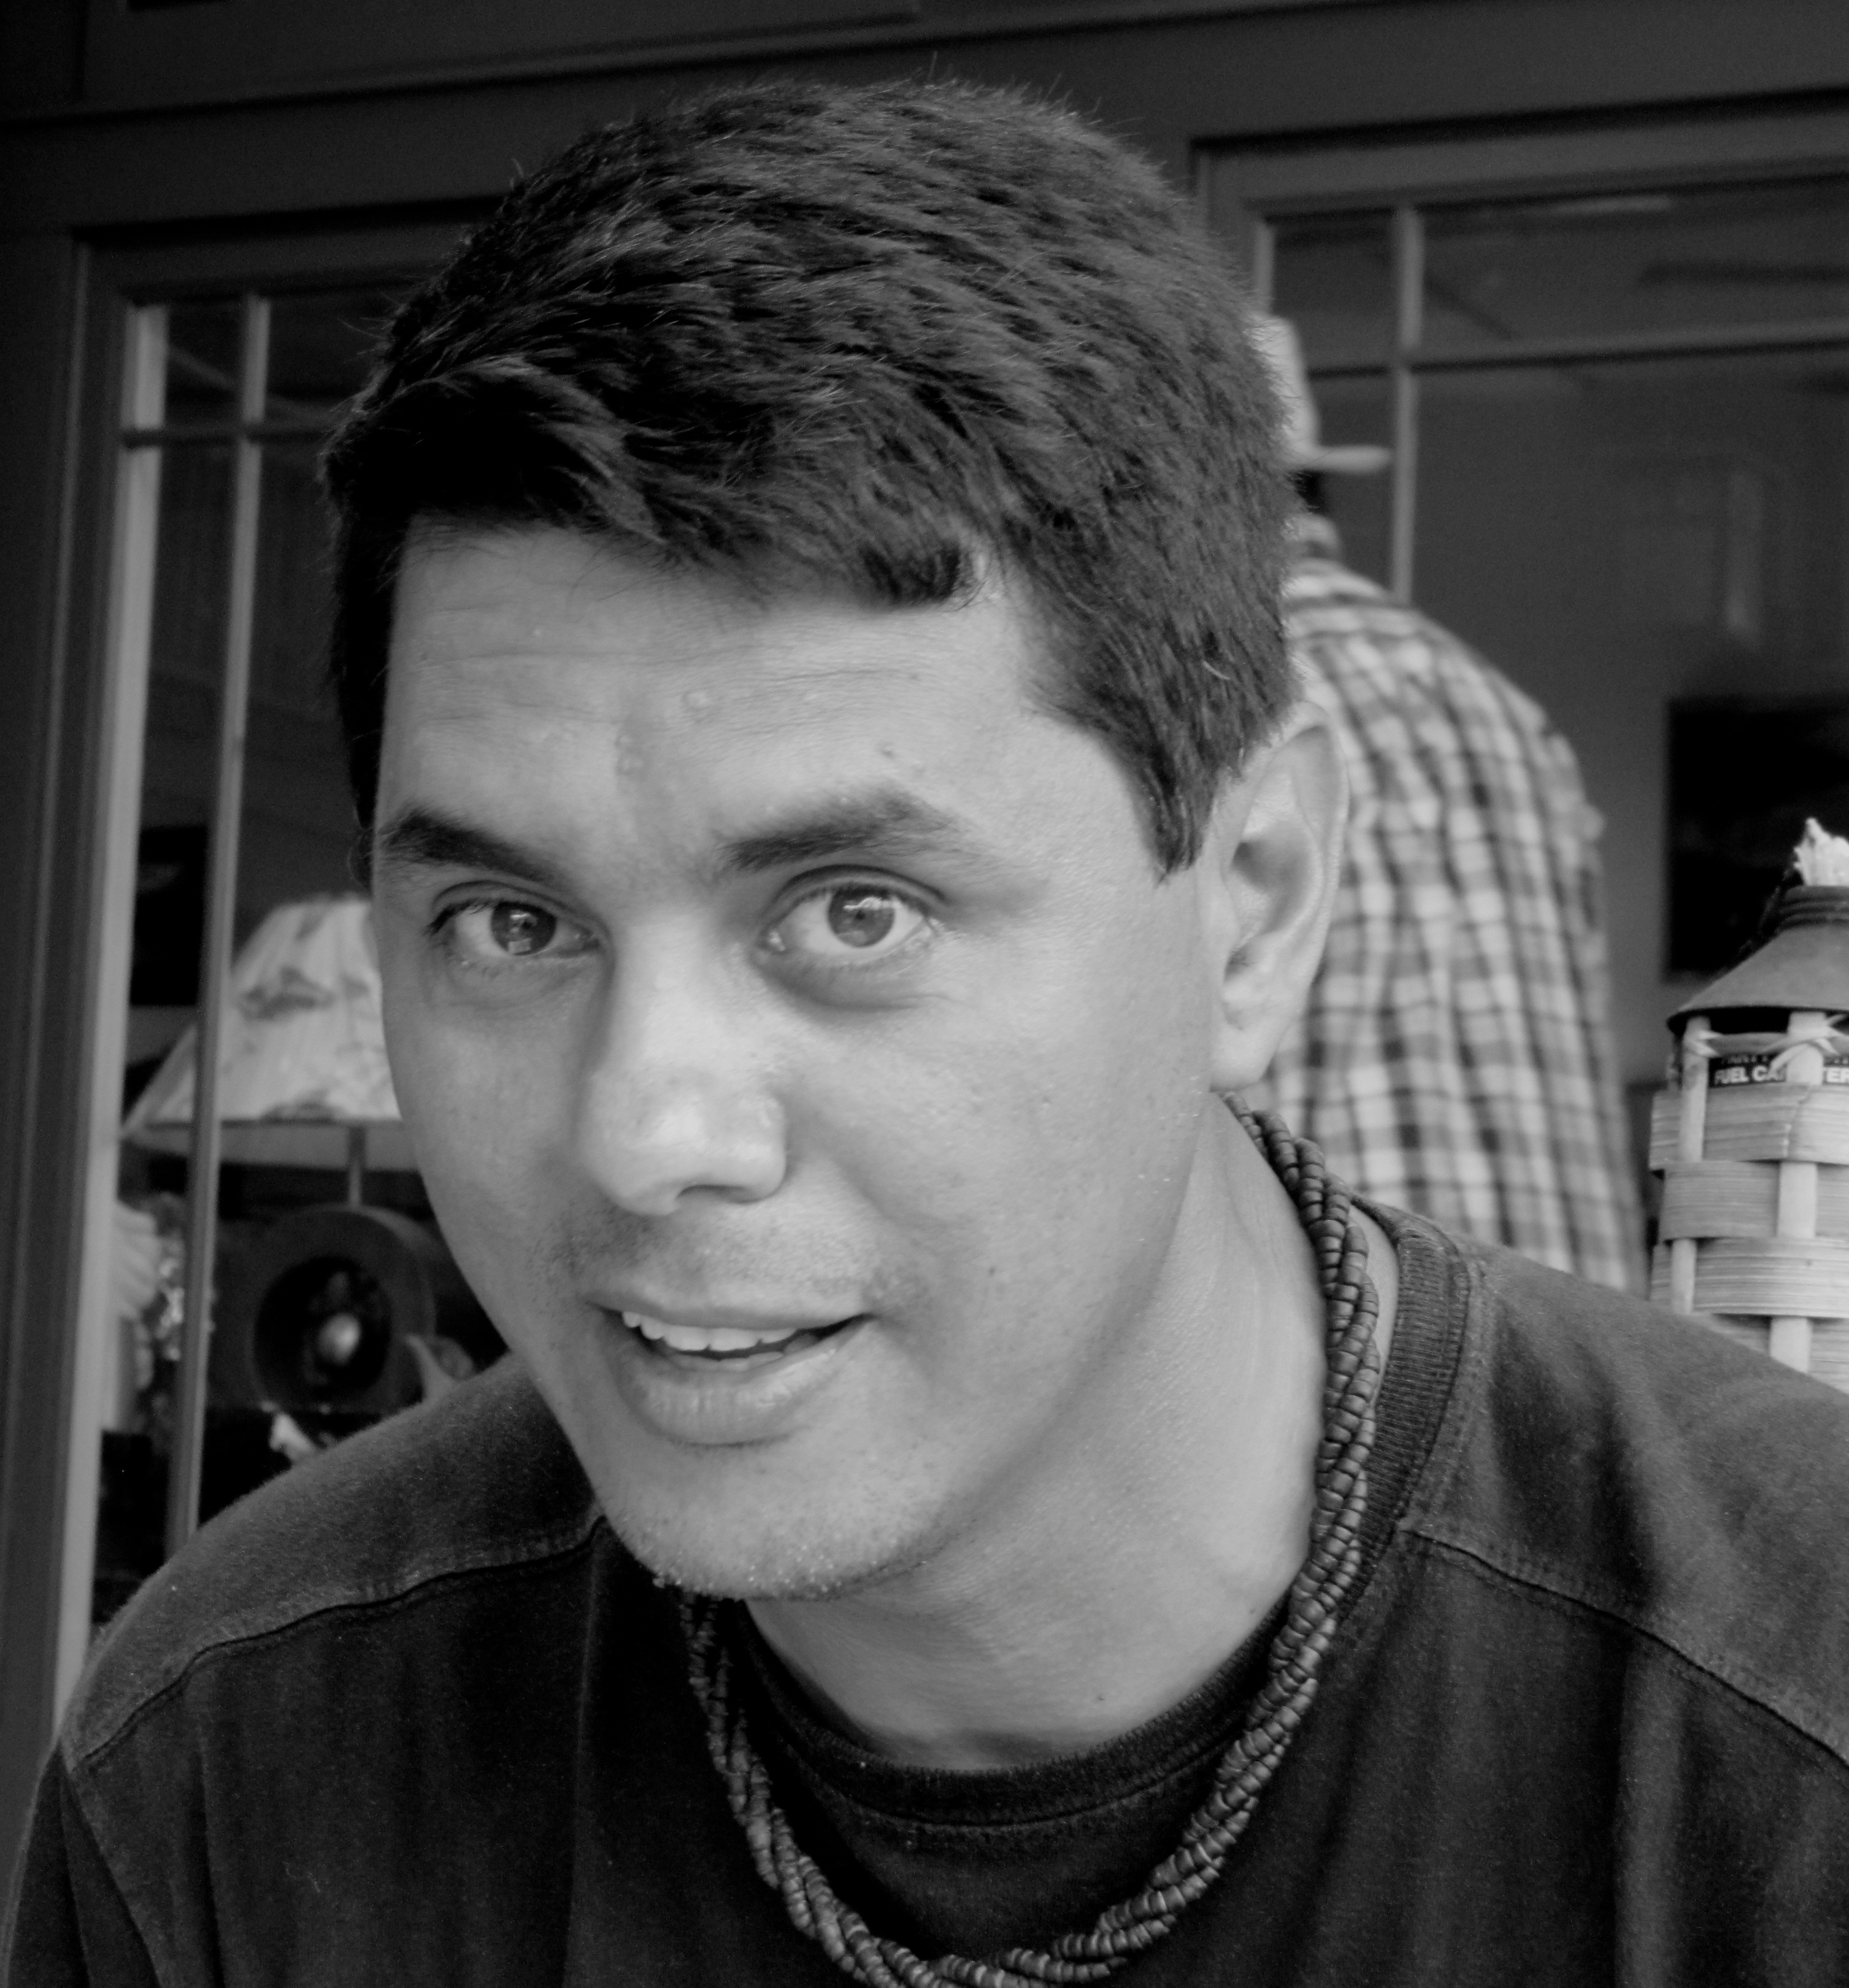
\includegraphics[width=0.35\textwidth]{./marco}			% Including picture
 		 \caption{Marco Reis em férias no Hawaii.}					% Caption of the figure
	\end{figure}														% End of the figure

Marco Reis tem 20 anos de experiência em gestão de projetos industriais, incluindo a participação na implantação de duas fábricas automotivas no Brasil (Renault em Curitiba-PR e Ford em Camaçari-BA), assim como passagens nas indústrias siderúrgicas e de geração de energia. Marco desenvolveu projetos nas áreas de gerenciamento de ativos e engenharia de confiabilidade, no desenvolvimento de ferramentas robóticas e veículos autônomos. Marco é formado em engenharia elétrica pela UFPR e mestrado em engenharia de produção pela UFSC. Atualmente lidera o grupo do Instituto Brasileiro de Robótica (BIR) em parceria com o Centro Alemão de Inteligência Artificial (DFKI) e coordena dois projetos de robótica autônoma no Senai Cimatec nas áreas de inspeção de linhas de transmissão de 138kV e de estruturas subaquáticas.
